

%----------------------------------------------------------------------------------------
%	PACKAGES AND DOCUMENT CONFIGURATIONS
%----------------------------------------------------------------------------------------

\documentclass[a4paper,12pt]{article}
\usepackage[margin=1in]{geometry}
\renewcommand{\baselinestretch}{1.2}
\usepackage{siunitx} % Provides the \SI{}{} and \si{} command for typesetting SI units
\usepackage{graphicx} % Required for the inclusion of images
\usepackage{subfigure}
\usepackage{multirow}
\usepackage{amsmath} % Required for some math elements 
\usepackage{indentfirst}
\usepackage{times} % Uncomment to use the Times New Roman font
\usepackage{appendix}
\usepackage{float}  
\usepackage{verbatim}
\renewcommand{\multirowsetup}{\centering}  


%----------------------------------------------------------------------------------------
%	DOCUMENT INFORMATION
%----------------------------------------------------------------------------------------

\title{\rule{\textwidth}{0.3mm} \\UM–SJTU JOINT INSTITUTE \\ PHYSICS LABORATORY \\ (VP241) \\ \rule{\textwidth}{0.3mm} \\ [30 mm]  \Large{Laboratory Report} \\[5 mm]  Exercise 5 \\[1 mm] 
RC, RL, and RLC Circuits \\[20 mm]} % Title
\author{Cao Zhiyuan} % Author name
\date{\today} % Date for the report

\begin{document}
\scshape

\maketitle % Insert the title, author and date

\begin{center}
\begin{tabular}{l l l}
\\[5 mm]
Partners:  \\
Name: Cao Zhiyuan & ID: 518370910030 & Group: 19 \\
~\\
Date Performed:\\
November 1, 2019\\
\end{tabular}
\end{center}

\thispagestyle{empty}


\newpage


\small\tableofcontents
\thispagestyle{empty}


\newpage

%----------------------------------------------------------------------------------------
%	SECTION 1
%----------------------------------------------------------------------------------------
\setcounter{page}{1}
\upshape
\section{\textsc{Objective}}
\begin{itemize}
\item Understand the physics of alternating-current circuits.
\item Learn the processes of charging/discharging of capacitors.
\item Understand the phenomenon of electromagnetic induction in inductive elements.
\item Investigate on other dynamic processes in RC, RL, and RLC series circuits.
\item Study the methods for measuring the amplitude-frequency.
\item Focus on the phase-frequency characteristics of RC, RL, and RLC series circuits.
\item Find the resonance frequency of a RLC circuit and its corresponding quality factor.
\end{itemize}

%----------------------------------------------------------------------------------------
%	SECTION 2
%----------------------------------------------------------------------------------------
\section{\textsc{Theoretical background}}
Resistors, capacitors, and inductors are the most basic elements in electric circuits. By choosing different arrangement of these elements, such as RC, RL, RLC, etc., the alternating-current is able to display different features, including transient, steady state, and resonant behavior.
\subsection{\textsc{Transient Processes in RC, RL, RLC Series Circuits}}
\subsubsection{\textsc{RC Series Circuits}}
In a RC circuit, transient process refers to the process of charging or discharging of a capacitor. As shown in Fig.1, a RC series circuit is connected with a square-wave input signal.

\begin{figure}[htb] 
    \centering
    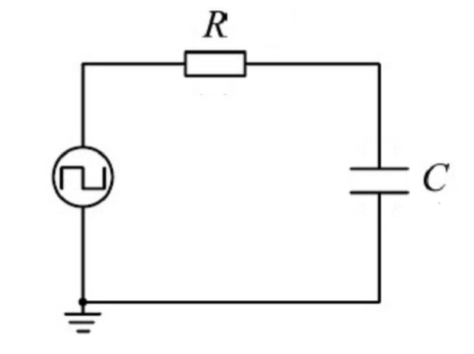
\includegraphics[width=0.4\textwidth]{Fig1} 
    \caption{RC series circuit. \cite{labmanual}} 
\end{figure}

In the first part of one period, the voltage of the square-wave is $U(t)=\mathcal{E}$, and as a result the capacitor is charged. In the second part of one period, the voltage of the square-wave is $U(t)=0$, and the capacitor is discharged. Then, we are able to use Kirchhoff’s Voltage Law to write down the following equation:
\begin{equation}
R C \frac{\mathrm{d} U_{C}}{\mathrm{d} t}+U_{C}=\mathcal{E}
\end{equation}
Also, if we take into consideration the initial condition:
\begin{center}
$U_{C}(t=0)=0$
\end{center}
we are able to find out the solution of Eq.(1):
\begin{center}
$U_{C}=\mathcal{E}\left(1-e^{-\frac{t}{R C}}\right) \quad \text { and } \quad U_{R}=i R=\mathcal{E} e^{-\frac{t}{R C}}$
\end{center}
Hence, we can see that the voltage across the capacitor increases exponentially with time, while the voltage on the resistor decreases exponentially. Fig.2 shows the different situation for the voltages.

\begin{figure}[htb] 
    \centering
    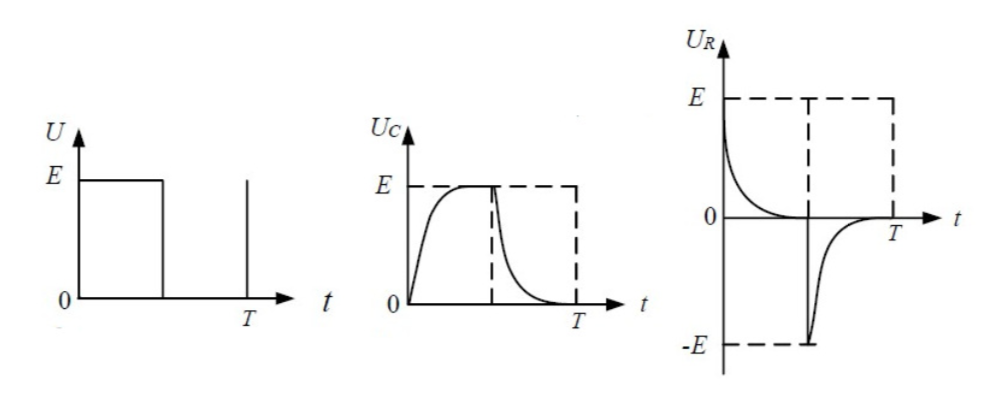
\includegraphics[width=0.9\textwidth]{Fig2} 
    \caption{Charging/discharging curves for a RC series circuit. \cite{labmanual}} 
\end{figure}

On the other hand, for the discharging process, we have the following equation based on Kirchhoff’s Voltage Law:
\begin{equation}
R C \frac{\mathrm{d} U_{C}}{\mathrm{d} t}+U_{C}=0
\end{equation}
Also, if we take into consideration the initial condition:
\begin{center}
$U_{C}(t=0)=\mathcal{E}$
\end{center}
we are able to find out the solution of Eq.(1):
\begin{center}
$U_{C}=\mathcal{E} e^{-\frac{t}{R C}} \quad \text { and } \quad U_{R}=i R=-\mathcal{E} e^{-\frac{t}{R C}}$
\end{center}
where both the voltage across the capacitor and the resistor decreases exponentially with time. Observing the solutions, since $\tau = RC$ has units of time, it is defined as the \textbf{time constant}, characterizing the dynamics of the transient process.
\par At the same time, another characteristics related to the time constant is called the \textbf{half-life period} $T_{1/2}$. It is important because it is easy to measure in experiments. Half-life period refers to the time needed for the voltage across the capacitor to decrease to a half of the initial value or increase to a half of the terminal value. In all, the quantities are related by the following equation:
\begin{center}
$\displaystyle T_{\frac{1}{2}}=\tau \ln 2 \approx 0.693 \tau$
\end{center}


\subsubsection{\textsc{RL Series Circuits}}
Similar to the RC case, in RL series circuits, we have the following results:
\begin{center}
$\displaystyle \tau = \frac{L}{R}$\\
\end{center}
and
\begin{center}
$\displaystyle T_{\frac{1}{2}}=\frac{L}{R} \ln 2$
\end{center}


\subsubsection{\textsc{RLC Series Circuits}}
To begin with, we discuss the case when a power source is plugged into a RLC circuit. We know that the voltage across the capacitor will satisfy the KVL law.
\begin{equation}
L C \frac{\mathrm{d}^{2} U_{C}}{\mathrm{d} t^{2}}+R C \frac{\mathrm{d} U_{C}}{\mathrm{d} t}+U_{C}=\mathcal{E}
\end{equation} 
Eq.(3) can be rewritten as:
\begin{equation}
\frac{\mathrm{d}^{2} U_{C}}{\mathrm{d} t^{2}}+2 \beta \frac{\mathrm{d} U_{C}}{\mathrm{d} t}+\omega_{0}^{2} U_{C}=\omega_{0}^{2} \mathcal{E}
\end{equation}
with 
\begin{center}
$\displaystyle \beta=\frac{R}{2 L}$ 
\end{center}
and 
\begin{center}
$\displaystyle \omega_{0}=\frac{1}{\sqrt{L C}}$ 
\end{center}

Note that Eq.(3) is a inhomogeneous differential equation, which is mathematically equivalent to the equation of motion of a damped harmonic oscillator with a constant driving force. Hence, we are able to make an analogue to the scenario of a damped harmonic oscillator, where $\beta$ is the damping coefficient and $\omega_0$ refers to the natural angular frequency. 
\par Given the following initial conditions:
\begin{center}
$\displaystyle U_{C}(t=0)=0$ 
\end{center}
and 
\begin{center}
$\displaystyle \left.\frac{\mathrm{d} U_{C}}{\mathrm{d} t}\right|_{t=0}=0$ 
\end{center}
we are able to find out its solution depending on the relationship between $\beta$ and $\omega_0$:
\begin{itemize}
\item In the \textbf{weak damping/ underdamped} case, where $\beta^{2}-\omega_{0}^{2}<0$, the system is in the underdamped regime and the solution can be written as:
	\begin{center}
	$U_{C}=\mathcal{E}-\mathcal{E} e^{-\beta t}\left(\cos \omega t+\frac{\beta}{\omega} \sin \omega t\right)$
	\end{center}
	where $\omega=\sqrt{\omega_{0}^{2}-\beta^{2}}$.
\item In the \textbf{strong damping/ overdamped} case, where $\beta^{2}-\omega_{0}^{2}>0$, the system is in the overdamped regime and the solution can be written as:
	\begin{center}
	$U_{C}=\mathcal{E}-\frac{\mathcal{E}}{2 \gamma} e^{-\beta t}\left[(\beta+\gamma) e^{\gamma t}-(\beta-\gamma) e^{-\gamma t}\right]$
	\end{center}
	where $\gamma=\sqrt{\beta^{2}-\omega_{0}^{2}}$.
\item In the \textbf{critically damped} case, where $\beta^{2}-\omega_{0}^{2}=0$, the solution can be written as:
	\begin{center}
	$U_{C}=\mathcal{E}-\mathcal{E}(1+\beta t) e^{-\beta t}$
	\end{center}
\end{itemize}
When the system has reached its steady state, if the power source is suddenly removed, or the switch is disconnected, the differential equations are similar to those we have discussed above, and there are also three different regimes. 
\par It should be noted that the above discussion is only valid for an ideal circuit where a step-signal source has zero internal resistance. However, in the real experiment, a square-wave source with a small internal resistance is used. As a result, the period of the square-signal must be much larger than the time constant. Also, the voltage across the capacitor will finally reach $\mathcal{E}$ no matter what the regime is. The situations are shown in Fig.3.

\begin{figure}[htb] 
    \centering
    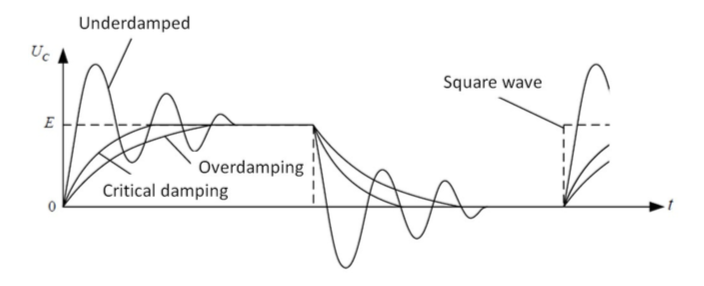
\includegraphics[width=0.9\textwidth]{Fig3} 
    \caption{Three different regimes of transient processes in a RLC series circuit. \cite{labmanual}} 
\end{figure}

\subsection{\textsc{RC, RL Steady–State Circuits}}
When sinusoidal ac input voltage is supplied to a RC(or RL) series circuit, the magnitude and phase of the voltage between the capacitor and the resistor will vary with the frequency of the input voltage. After that, the amplitude vs. frequency relation and the phase vs. frequency relation can be measured among the following equations:
\begin{center}
$\displaystyle \varphi=\tan ^{-1}\left(\frac{U_{L}}{U_{R}}\right)=\tan ^{-1}\left(\frac{\omega L}{R}\right)$
\end{center}
and 
\begin{center}
$\displaystyle \varphi=\tan ^{-1}\left(-\frac{U_{C}}{U_{R}}\right)=\tan ^{-1}\left(-\frac{1}{\omega R C}\right)$
\end{center}

\subsection{\textsc{RLC Resonant Circuit}}
\subsubsection{\textsc{RLC Series Circuit}}
RLC series circuits refer to the circuits where the capacitor, inductor, and resistor are connected in series. The circuit is shown in Fig.4. Then, we can express capacitor, inductor and resistor in terms of phasor domain. In other words, the phase differences between them can be expressed as:
\begin{center}
$\displaystyle \varphi_{R}=0, \quad \varphi_{L}=\frac{\pi}{2}, \quad \varphi_{C}=-\frac{\pi}{2}$
\end{center}

\begin{figure}[htb] 
    \centering
    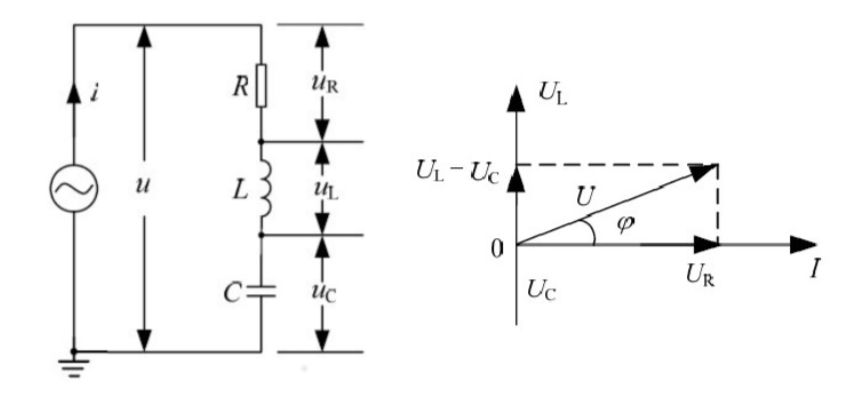
\includegraphics[width=0.9\textwidth]{Fig4} 
    \caption{RLC series circuit. \cite{labmanual}} 
\end{figure}

Then,  the voltage amplitudes can be written as follows:
\begin{center}
$\displaystyle U_{R}=I Z=I R, \quad U_{L}=I Z_{L}=I \omega L, \quad U_{C}=I Z_{C}=\frac{I}{\omega C}$
\end{center}

Therefore the amplitude of voltage and total impedance can be expressed as follows respectively:
\begin{equation}
U=\sqrt{U_{R}^{2}+\left(U_{L}-U_{C}\right)^{2}} \quad \text { or } \quad U=I \sqrt{R^{2}+\left(\omega L-\frac{1}{\omega C}\right)^{2}}
\end{equation}
and 
\begin{equation}
Z=\sqrt{R^{2}+\left(\omega L-\frac{1}{\omega C}\right)^{2}}
\end{equation}

The phase difference is:
\begin{equation}
\varphi=\tan ^{-1}\left(\frac{U_{L}-U_{C}}{U_{R}}\right)=\tan ^{-1}\left(\frac{\omega L-\frac{1}{\omega C}}{R}\right)
\end{equation}

\subsubsection{\textsc{Resonance}}
It can be verified that the total impedance will reach minimum $Z_m = R$ if the following condition is satisfied:
\begin{center}
$\displaystyle \omega_0 = \frac{1}{\sqrt{LC}}$
\end{center}
Note that the actual value of the resistance R in the actual circuit will be greater than the theoretical value because it includes the internal resistance and the power loss of various ac currents.
\par The circuit is in the state of resonance if its current reaches maximum. The frequency can be expressed as:
\begin{center}
$\displaystyle f_{0}=\frac{\omega_{0}}{2 \pi}=\frac{1}{2 \pi \sqrt{L C}}$
\end{center}
which is called resonance frequency.
\par Fig.5 shows the dependence of the total impedance, current, and phase difference on the frequency respectively. Based on our calculations in Eq.(5) and (6), the following cases occur:
\begin{itemize}
\item if frequency is low (i.e. $f<f_0$ and $1/\omega C > \omega L$), we have $\varphi < 0$. In this case, voltage lags behind the current and the circuit is capacitive.
\item if frequency is resonant (i.e. $f=f_0$ and $1/\omega C = \omega L$), we have $\varphi = 0$. In this case, the voltage and the current equals to each other and the circuit is resistive.
\item if frequency is high (i.e. $f>f_0$ and $1/\omega C < \omega L$), we have $\varphi > 0$. In this case, voltage leads the current and the circuit is inductive.
\end{itemize}

\begin{figure}[htb] 
    \centering
    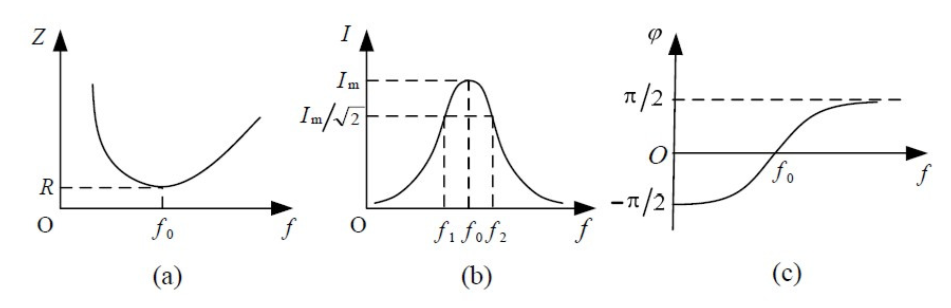
\includegraphics[width=1\textwidth]{Fig5} 
    \caption{The impedance, the current and the phase difference as functions of the fre- quency for a RLC series circuit (generic sketches). \cite{labmanual}} 
\end{figure}

\subsubsection{\textsc{Quality Factor in Resonant Circuits}}
Since in the phasor domain the Ohm's Law still holds, the voltages across the resistor, the inductor, and the capacitor can be written as follows:
\begin{center}
$\displaystyle U_R = I_m R = U$\\
$\displaystyle U_{L} =I_{\mathrm{m}} Z_{L}=\frac{U}{R} \omega L$ \\ 
$\displaystyle U_{C} =I_{\mathrm{m}} Z_{C}=\frac{U}{R} \frac{1}{\omega_{0} C}=U_{L}$ 
\end{center}

For a circuit at the resonant state, the ratio of $U_L$/$U_C$ to $U$ is called the quality factor Q 
\begin{center}
$\displaystyle Q=\frac{U_{L}}{U}=\frac{\omega_{0} L}{R} \quad \text { or } \quad Q=\frac{U_{C}}{U}=\frac{1}{\omega_{0} R C}$
\end{center}
\par If we fix the total voltage, then $U_L$ and $U_C$ will increase with the increase of $Q$. And Q is used to examine the efficiency of resonant circuits.
\par We can express the quality factor through the following formula:
\begin{equation}
Q = \frac{f_0}{f_2 - f_1}
\end{equation}
where $f_1$ and $f_2$ are the frequencies enabling $\displaystyle I(f_1) = I(f_2) = \frac{I_m}{\sqrt{2}}$. Details are shown in Fig.5b.
%----------------------------------------------------------------------------------------
%	SECTION 3
%----------------------------------------------------------------------------------------
\section{\textsc{Apparatus and Experimental Setup}}
In this lab, we use the following apparatuses:
\begin{itemize}
\item A signal generator
\item An oscilloscope
\item A digital multimeter
\item A wiring board
\item A fixed resistor 100 $\Omega$ (2 W)
\item A variable resistor 2 $k\Omega$ (2 W)
\item 0.47 $\mu F$ and 0.1 $\mu F$ capacitors
\item Two inductors (10 mH and 33 mH)
\end{itemize}

The uncertainties for the quantities measured in this lab are listed in Table 1:

\begin{table}[htbb]
\begin{center}
\begin{tabular}{|c|c|}
\hline
Quantity & Uncertainty \\ \hline
R        & 0.01 $\Omega$       \\ \hline
C        & 0.01 nF/ 0.1nF       \\ \hline
f        & 0.001 Hz      \\ \hline
$\mathcal{E}$     & 0.001 $V_{pp}$      \\ \hline
$T_{1/2}$        & 0.001 $\mu s$/ 0.01 $\mu s$      \\ \hline
L        & 0           \\ \hline
$U_R$        & 0.02 $V_{pp}$ /0.002 $V_{pp}$      \\ \hline
\end{tabular}
\caption{Uncertainties for quantities measured by apparatuses.}
\end{center}
\end{table}

Note that some of the uncertainties have two different values. This is due to the limitation of the apparatuses, and the choice of the uncertainty should based on our reading in lab.

%----------------------------------------------------------------------------------------
%	SECTION 4
%----------------------------------------------------------------------------------------
\section{\textsc{Procedures \cite{labmanual}}}
\subsection{\textsc{RC, RL Series Circuit}}
\begin{itemize}
\item[1.] We properly choose a capacitor and an inductor to build up a circuit with the 100$\Omega$ resistor.
\item[2.] We adjust the output frequency of the square wave signal provided by the signal generator.
\item[3.] We observe the waveform change when the time constant is less than or greater than the square-wave period. Then, we select the frequency at which the capacitor is allowed to fully charge/discharge.
\item[4.] We push the "PRINT" button on the oscilloscope or take a photo to record the waveforms.
\item[5.] We measure the $T_{1/2}$ for the circuit by adjusting the parameters on the oscilloscope.
\item[6.] Finally, we calculate the time constant and compare it with the theoretical value. Pay attention that only one period should be displayed on the oscilloscope.
\end{itemize}
\subsection{\textsc{RLC Series Circuit}}
\begin{itemize}
\item[1.] We properly choose a capacitor and an inductor to build up a RLC series circuit with variable resistor.
\item[2.] We observe the waveform of capacitor voltages in the underdamped, critically damped, and overdamped regimes respectively.
\item[3.] We push the "PRINT" button on the oscilloscope or take a photo to record the waveforms.
\item[4.] We adjust the variable resistor to the critically damped regime. Since we have $\beta T_{1/2} = 1.68$, we are able to find out time constant as $\tau=1 / \beta=T_{1 / 2} / 1.68$.
\end{itemize}
\subsection{\textsc{RLC Resonant Circuit}}
\begin{itemize}
\item[1.] To begin with we apply a sinusoidal input voltage $U_i$ to the RLC series circuit. Then, observe the change of the voltage $U_R$, and the phase difference between $U_R$ and $U_i$ for a fixed resistor R by changing the frequency.
\item[2.] After that, we measure how $U_R$ changes with $U_i$ and calculate the corresponding phase difference.
\item[3.] Finally, we plot the figures $I / I_{m} \text { vs. } f / f_{0} \text { and } \varphi \text { vs. } f / f_{0}$, and find out the resonance frequency and quality factor Q.
\end{itemize}

%----------------------------------------------------------------------------------------
%	SECTION 5
%----------------------------------------------------------------------------------------
\section{\textsc{Results}}
\subsection{\textsc{RC Series Circuit}}

\begin{table}[htbb]
\begin{center}
\begin{tabular}{|c|c|}
\hline
R & $99.90 [\Omega] \pm 0.01 [\Omega]$ \\ \hline
f & $ 5000.000 [Hz] \pm 0.001 [Hz] $ \\ \hline
$\mathcal{E}$ & $ 4.000[V_{pp}] \pm 0.001[V_{pp}] $ \\ \hline
C & $ 101.85 [nF] \pm 0.01 [nF] $ \\ \hline
$T_{1/2}$ & $ 8.000[\mu s] \pm 0.001[\mu s] $ \\ \hline
\end{tabular}
\caption{Measurement Data for a RC Series Circuit.}
\end{center}
\end{table}

\begin{figure}[htb] 
    \centering
    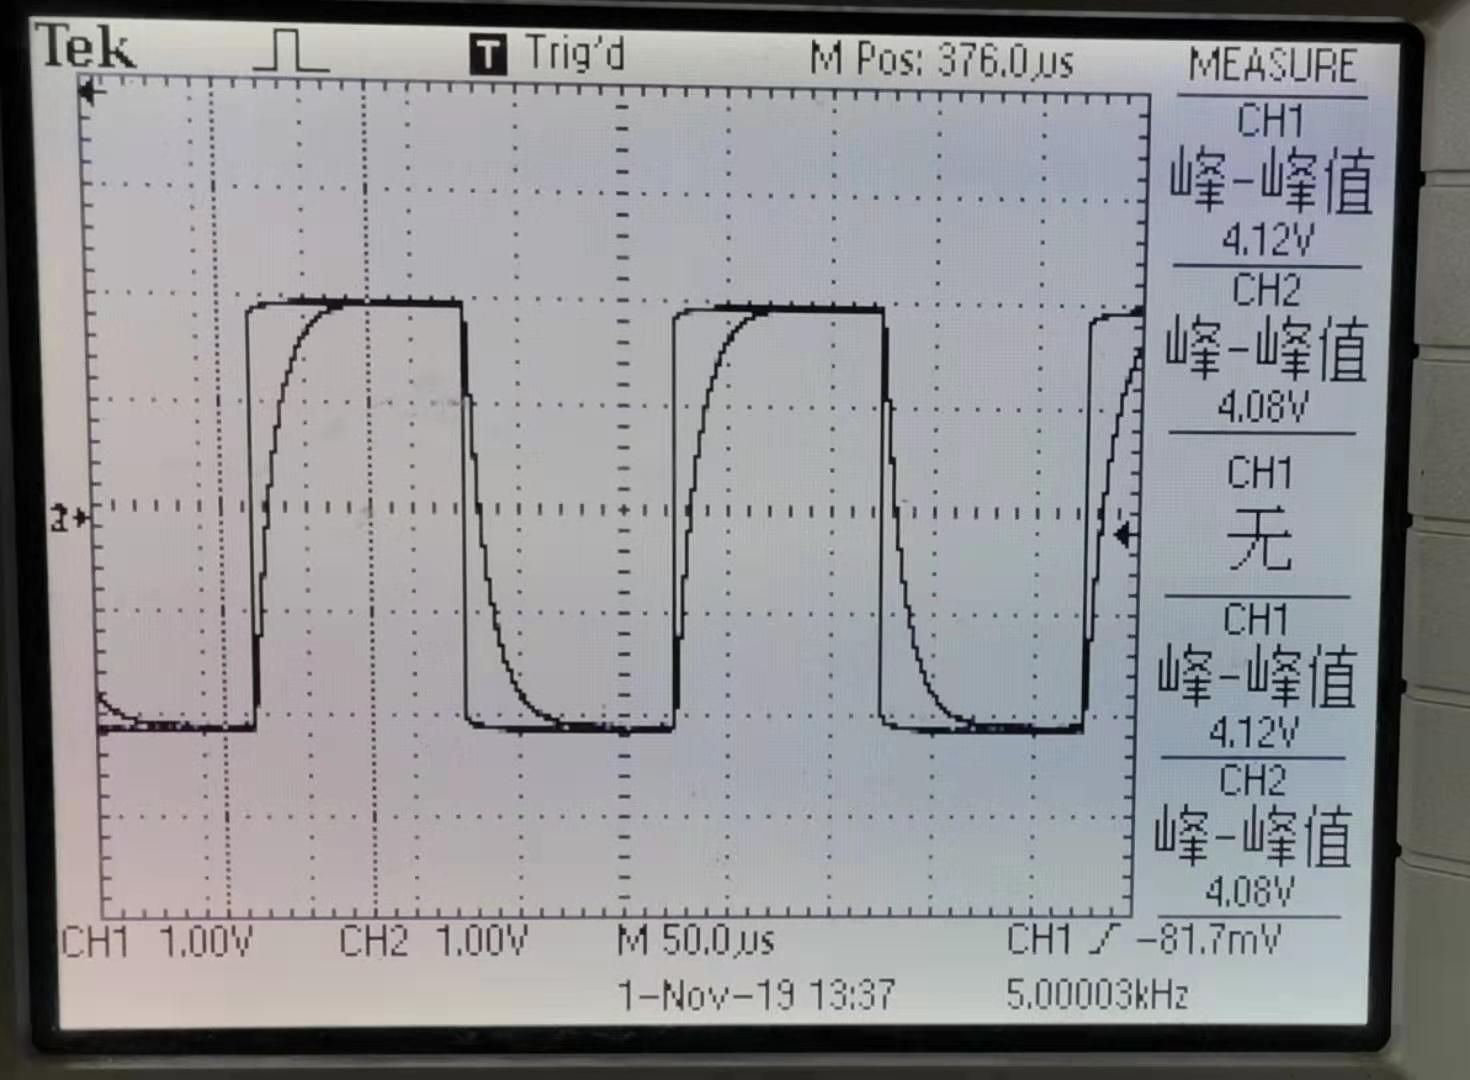
\includegraphics[width=0.7\textwidth]{p1} 
    \caption{Waveform for RC Series Circuit.} 
\end{figure}

\newpage
The data we obtain is recorded in Table 2, and the corresponding waveform on the oscilloscope is shown in Fig.6. Then, we are able to calculate the experimental time constant $\tau_{exp}$ and the theoretical time constant $\tau_{theo}$ respectively (Detailed calculations for uncertainties are shown in A.1.):
\begin{center}
$\displaystyle \tau_{exp} = \frac{T_{1/2}}{ln2} = \frac{8.000\times 10^{-6}}{0.693} = 1.15416 \times 10^{-5} \pm 0.00014 \times 10^{-5} [s]$
\end{center}
and
\begin{center}
$\tau_{theo} = RC = 99.90 \times 101.85 \times 10^{-9} = 1.01748 \times 10^{-5} \pm 0.00014 \times 10^{-5} [s] $
\end{center}
with a relative error 
\begin{center}
$\displaystyle u_\tau = \frac{1.15416 \times 10^{-5} - 1.01748 \times 10^{-5}}{1.01748 \times 10^{-5}} \times 100\% = 13\% $ 
\end{center}
which is relatively larger than expected. The reasons for such error will be discussed later.

\subsection{\textsc{RL Series Circuit}}

\begin{table}[htbb]
\begin{center}
\begin{tabular}{|c|c|}
\hline
R & $99.90 [\Omega] \pm 0.01 [\Omega]$ \\ \hline
f & $ 1000.000 [Hz] \pm 0.001 [Hz] $ \\ \hline
$\mathcal{E}$ & $ 4.000[V_{pp}] \pm 0.001[V_{pp}] $ \\ \hline
L & $ 0.01 [H] \pm 0 [H] $ \\ \hline
$T_{1/2}$ & $ 70.00[\mu s] \pm 0.01[\mu s] $ \\ \hline
\end{tabular}
\caption{Measurement Data for a RL Series Circuit.}
\end{center}
\end{table}

\begin{figure}[htb] 
    \centering
    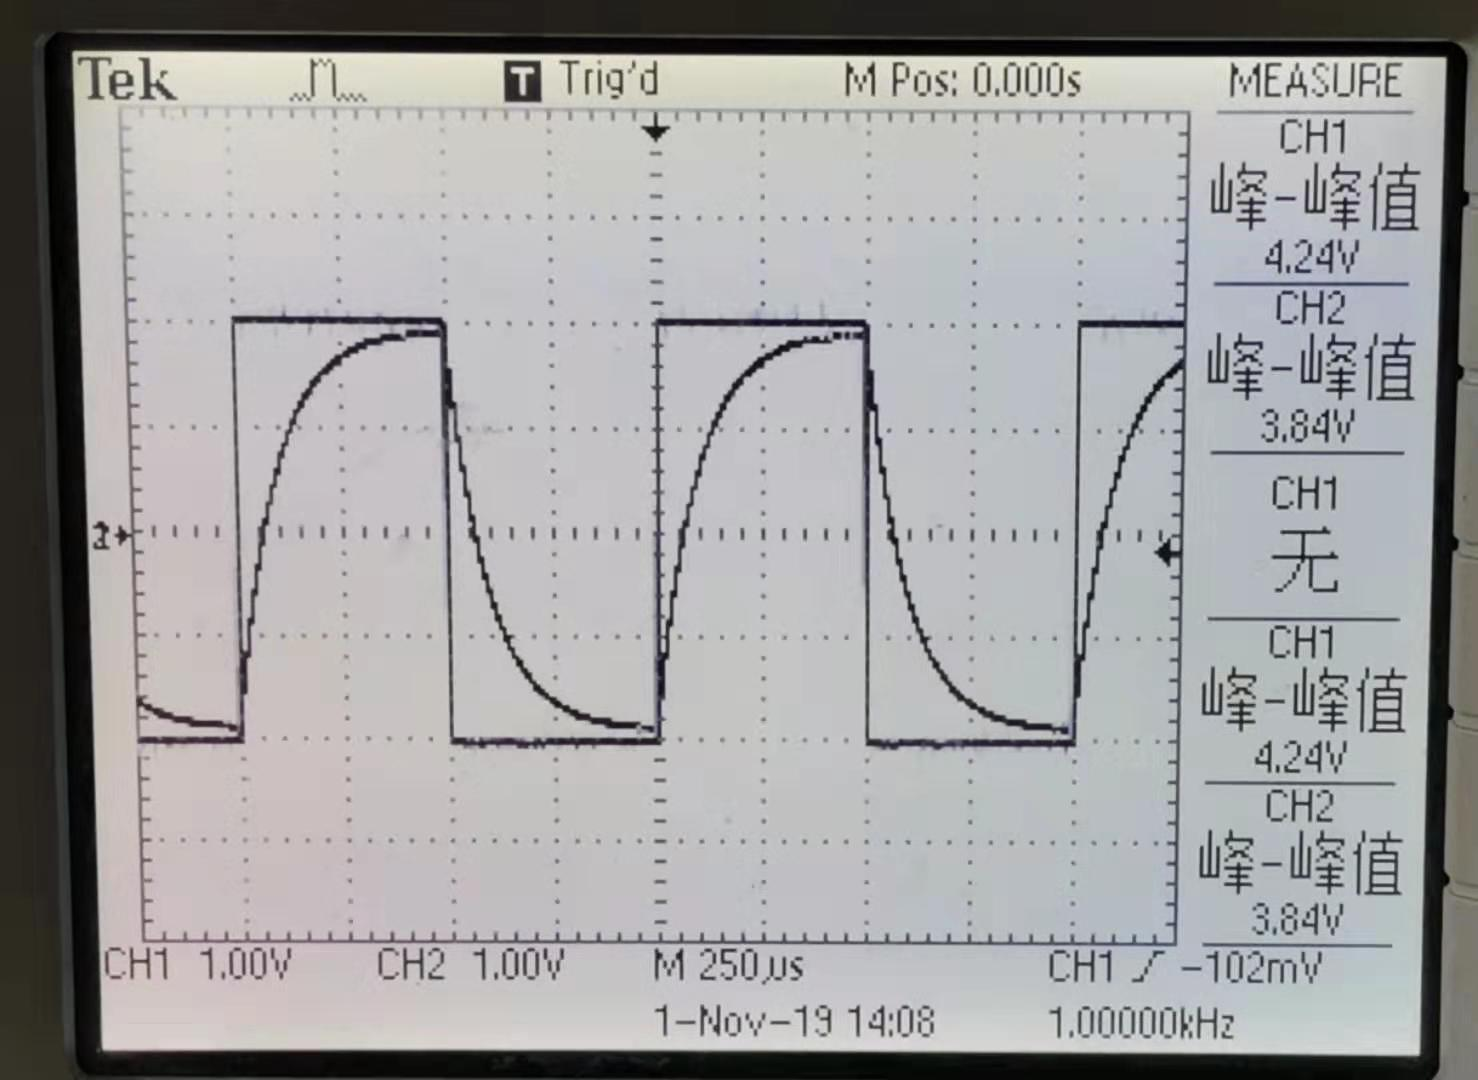
\includegraphics[width=0.7\textwidth]{p2} 
    \caption{Waveform for RL Series Circuit.} 
\end{figure}

\newpage
The data we obtain is recorded in Table 3, and the corresponding waveform on the oscilloscope is shown in Fig.7. Then, we are able to calculate the experimental time constant $\tau_{exp}$ and the theoretical time constant $\tau_{theo}$ respectively (Detailed calculations for uncertainties are shown in A.2.):
\begin{center}
$\displaystyle \tau_{exp} = \frac{T_{1/2}}{ln2} = \frac{70.00\times 10^{-6}}{0.693} = 1.00989 \times 10^{-4} \pm 0.00014 \times 10^{-4} [s]$
\end{center}
and
\begin{center}
$\displaystyle \tau_{theo} = \frac{L}{R} = \frac{0.01}{99.90} =  1.00100 \times 10^{-4} \pm 0.00010 \times 10^{-4} [s] $
\end{center}
with a relative error 
\begin{center}
$\displaystyle u_\tau = \frac{1.00989 \times 10^{-4} - 1.00100 \times 10^{-4}}{1.00100 \times 10^{-4}} \times 100\% = 0.9\% $ 
\end{center}
which is small, indicating that our experimental value is accurate.

\subsection{\textsc{RLC Series Circuit}}
\begin{table}[htbb]
\begin{center}
\begin{tabular}{|c|c|}
\hline
L & $0.01 [H] \pm 0 [H]$ \\ \hline
C & $ 101.85 [nF] \pm 0.01 [nF] $ \\ \hline
$\mathcal{E}$ & $ 4.000[V_{pp}] \pm 0.001[V_{pp}] $ \\ \hline
f & $ 1000.000 [Hz] \pm 0.001 [Hz] $ \\ \hline
$\beta t$ & $1.68$ \\ \hline
$T_{1/2}$ & $ 50.00[\mu s] \pm 0.01[\mu s] $ \\ \hline
\end{tabular}
\caption{Measurement Data for a RLC Series Circuit.}
\end{center}
\end{table}

\begin{figure}[H] 
	\centering  
	\vspace{-0.35cm} 
	\subfigtopskip=2pt %设置子图与上面正文或别的内容的距离
	\subfigbottomskip=5pt %设置第二行子图与第一行子图的距离,即下面的头与上面的脚的距离
	\subfigcapskip=-5pt %设置子图与子标题之间的距离
	\subfigure[Underdamped]{
		\label{level.sub.1}
		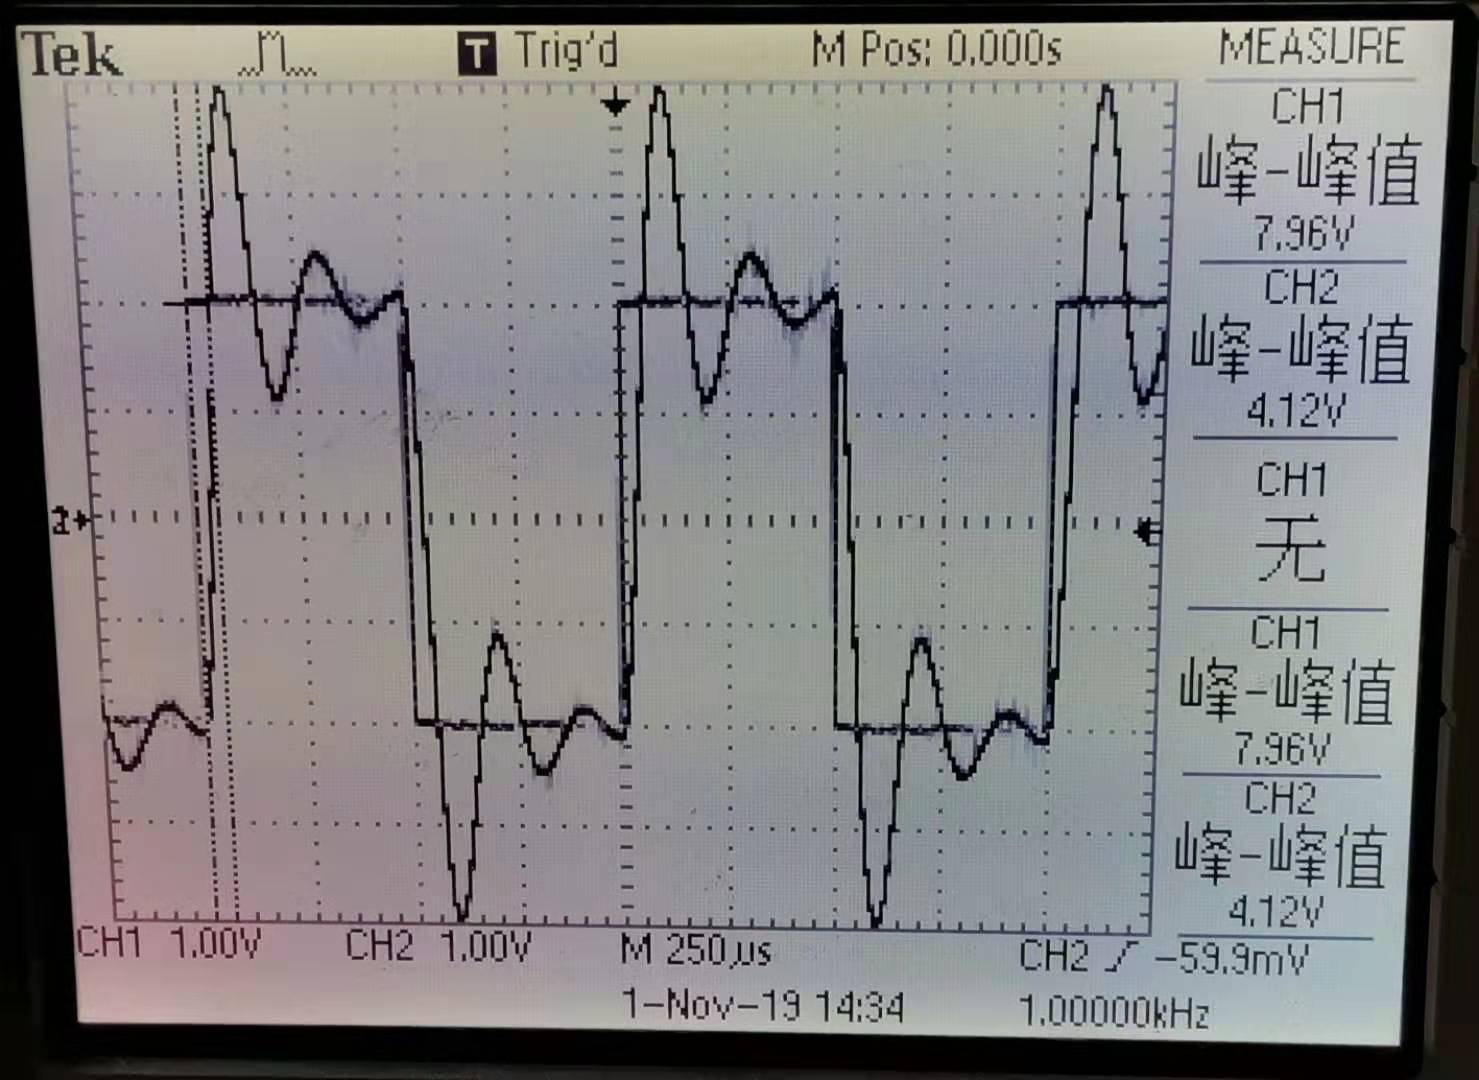
\includegraphics[width=0.6\linewidth]{p3}}
		
	\subfigure[Critically damped]{
		\label{level.sub.3}
		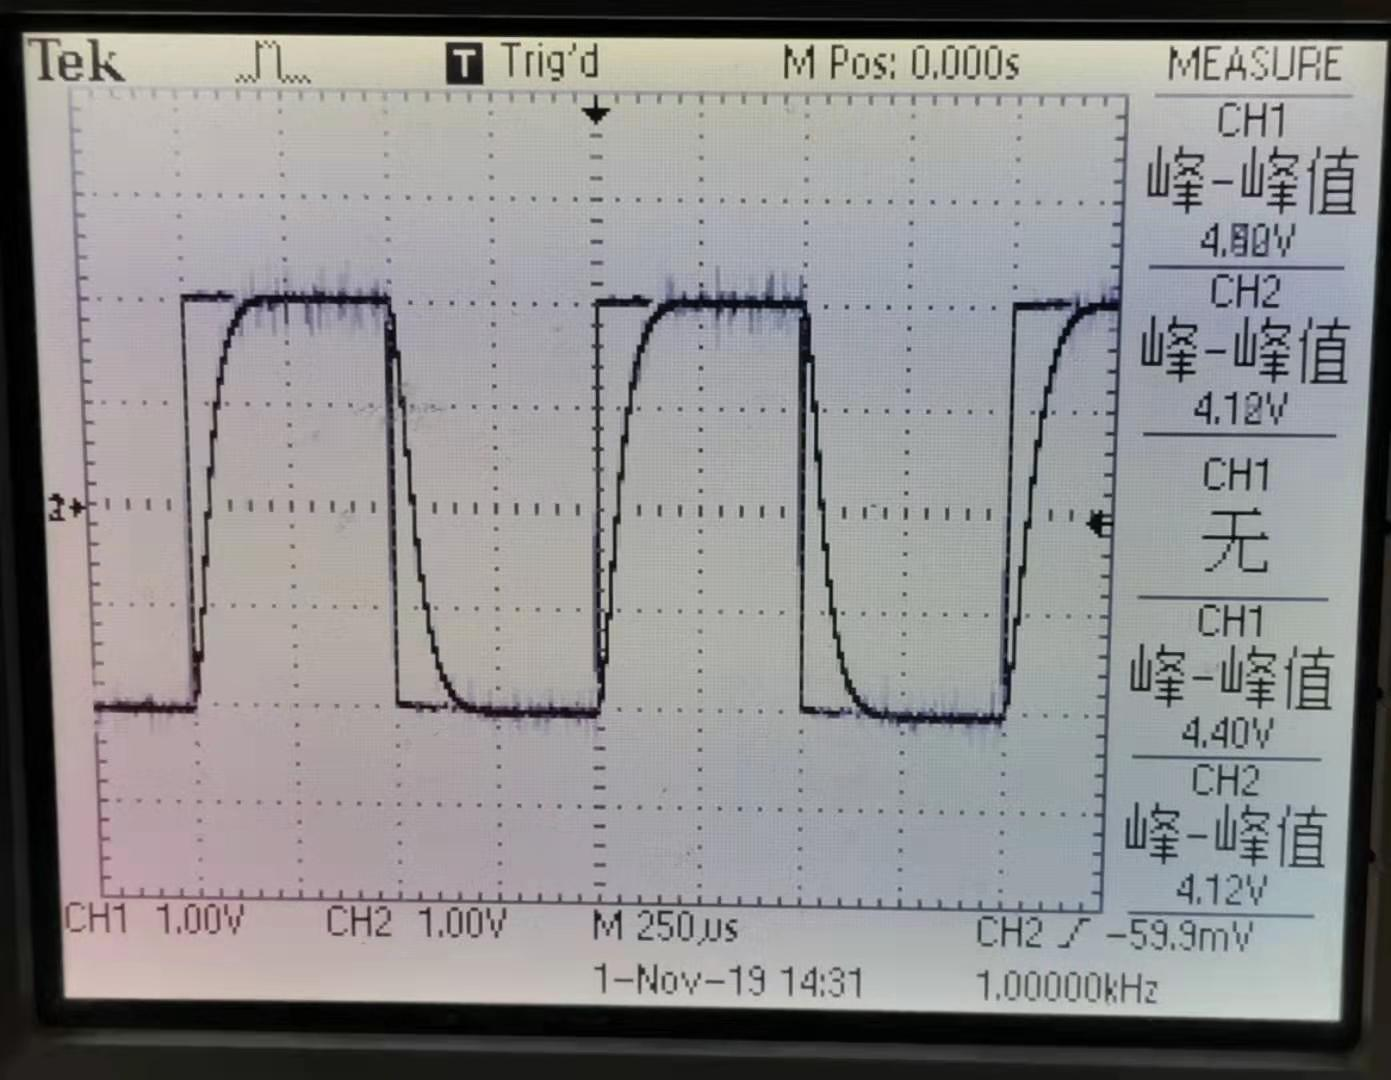
\includegraphics[width=0.6\linewidth]{p4}}
		
	\subfigure[Overdamped]{
		\label{level.sub.3}
		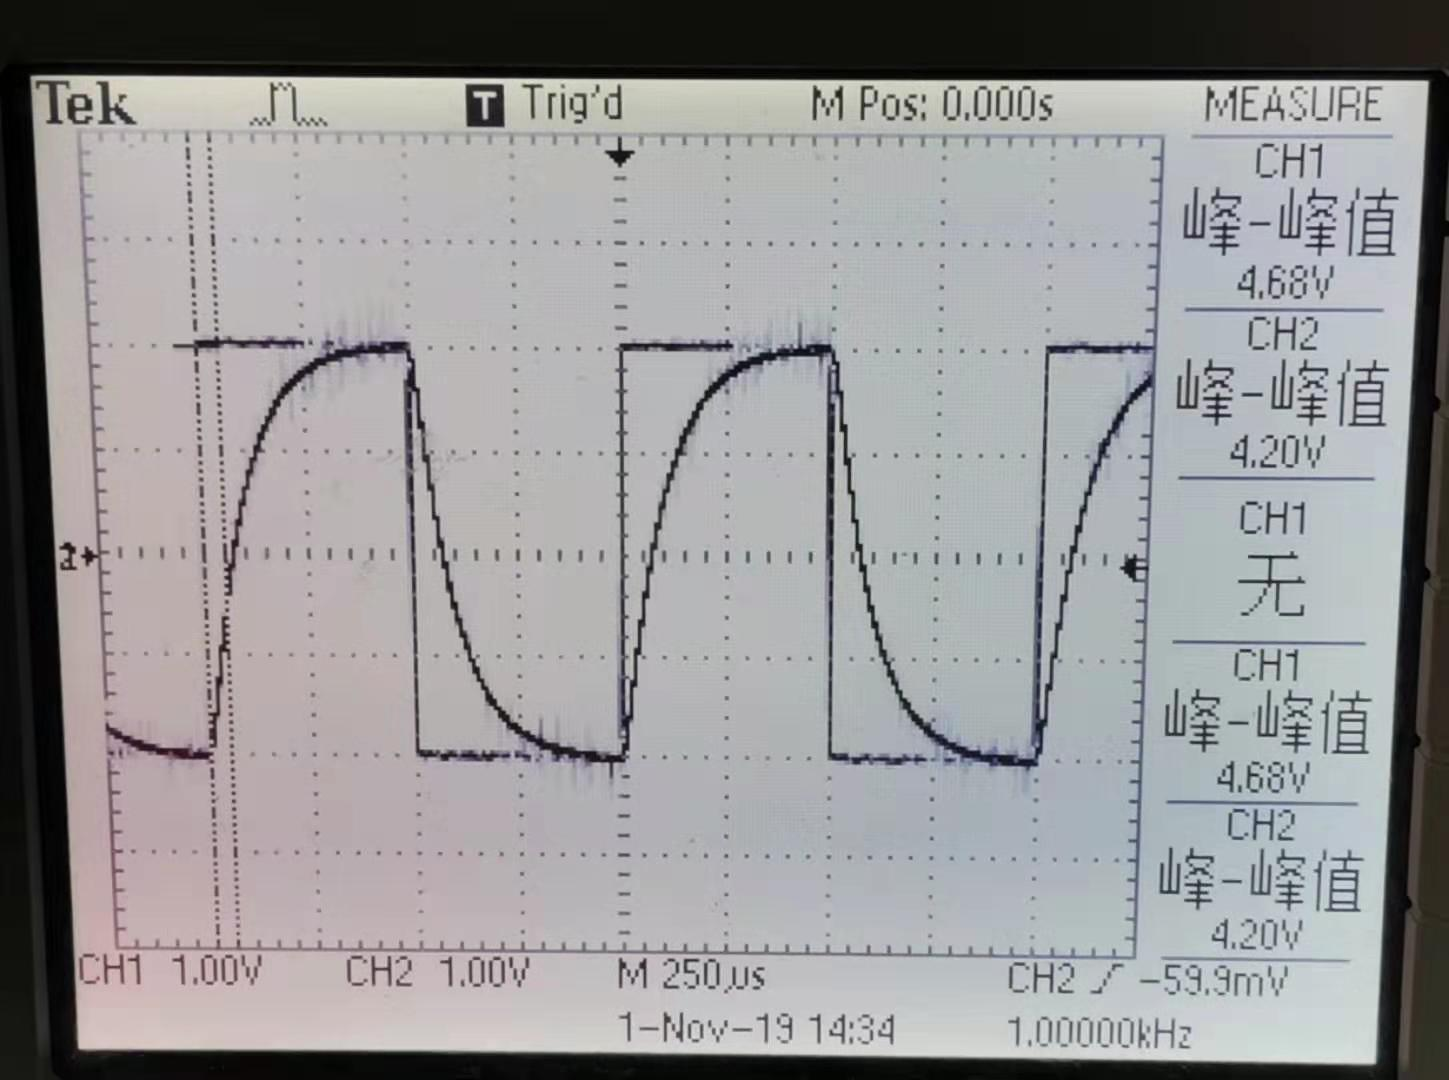
\includegraphics[width=0.6\linewidth]{p5}}
	\caption{Waveforms for RLC Series Circuit.}
	\label{level}
\end{figure}

The data we obtain is recorded in Table 4, and the corresponding waveforms on the oscilloscope are shown in Fig.8. Then, we are able to calculate the experimental time constant $\tau_{exp}$ and the theoretical time constant $\tau_{theo}$ respectively (Detailed calculations for uncertainties are shown in A.3.):
\begin{center}
$\displaystyle \tau_{exp} = \frac{T_{1/2}}{\beta t} = \frac{50.00\times 10^{-6}}{1.68} = 2.9762 \times 10^{-5} \pm 0.0006 \times 10^{-5} [s]$
\end{center}
and
\begin{center}
$\displaystyle \tau_{theo} = \sqrt{LC} = \sqrt{0.01\times 101.85 \times 10^{-9}} =  3.19139 \times 10^{-5} \pm 0.00016 \times 10^{-5} [s] $
\end{center}
with a relative error 
\begin{center}
$\displaystyle u_\tau = \frac{2.9762 \times 10^{-5} - 3.19139 \times 10^{-5}}{3.19139 \times 10^{-5}} \times 100\% = -7\% $ 
\end{center}
which is a little large, but acceptable. This indicate that our experimental value is wroth learning. The errors will be discussed later.

\subsection{\textsc{RLC Resonant Circuit}}
\subsubsection{\textsc{Amplitude-frequency characteristic}}

\begin{table}[htbb]
\begin{center}
\begin{tabular}{|c|c|}
\hline
$ R = 99.90 [\Omega] \pm 0.01 [\Omega] $      & $L = 0.01 [H]\pm 0 [H]$                    \\ \hline
$ C = 101.85 [nF] \pm 0.01 [nF] $             & $ f_0 = 5100.000[Hz] \pm 0.001 [Hz] $      \\ \hline
\multicolumn{2}{|c|}{$ \mathcal{E}  = 4.000 [V_{pp}] \pm 0.001[V_{pp}] $}                   \\ \hline
\end{tabular}
\caption{Other uncertainties for RLC resonant circuit.}
\end{center}
\end{table}


\begin{table}[p]
\begin{center}
\begin{tabular}{|c|c|c|c|c|c|}
\hline
$U_R [V_{pp}] \pm 0.02 [V_{pp}] $  & f$[Hz] \pm 0.001[Hz]$ & $I/I_m$                       & $u_{I/I_m}$                      & $f/f_0$                           & $u_{f/f_0}$                          \\ \hline
1.00                       & 2700.000                      & 0.258                      & 0.005                      & 0.5294118                      & 0.0000002                      \\ \hline
1.32                       & 3200.000                      & 0.340                      & 0.005                      & 0.6274510                      & 0.0000002                      \\ \hline
1.88                       & 3700.000                      & 0.485                      & 0.006                      & 0.7254902                      & 0.0000002                      \\ \hline
2.44                       & 4100.000                      & 0.629                      & 0.006                      & 0.8039216                      & 0.0000003                      \\ \hline
2.84                       & 4300.000                      & 0.732                      & 0.006                      & 0.8431373                      & 0.0000003                      \\ \hline
3.04                       & 4400.000                      & 0.784                      & 0.007                      & 0.8627451                      & 0.0000003                      \\ \hline
3.40                       & 4600.000                      & 0.876                      & 0.007                      & 0.9019608                      & 0.0000003                      \\ \hline
3.56                       & 4700.000                      & 0.918                      & 0.007                      & 0.9215686                      & 0.0000003                      \\ \hline
3.72                       & 4800.000                      & 0.959                      & 0.007                      & 0.9411765                      & 0.0000003                      \\ \hline
3.80                       & 4900.000                      & 0.979                      & 0.007                      & 0.9607843                      & 0.0000003                      \\ \hline
\multicolumn{1}{|c|}{3.84} & \multicolumn{1}{c|}{5000.000} & \multicolumn{1}{c|}{0.990} & \multicolumn{1}{l|}{0.007} & \multicolumn{1}{l|}{0.9803921} & \multicolumn{1}{l|}{0.0000003} \\ \hline
3.88                       & 5100.000                      & 1.000                      & 0.007                      & 1.0000000                      & 0.0000003                      \\ \hline
3.84                       & 5150.000                      & 0.990                      & 0.007                      & 1.0098039                      & 0.0000003                      \\ \hline
3.72                       & 5250.000                      & 0.959                      & 0.007                      & 1.0294118                      & 0.0000003                      \\ \hline
3.56                       & 5400.000                      & 0.918                      & 0.007                      & 1.0588235                      & 0.0000003                      \\ \hline
3.24                       & 5600.000                      & 0.835                      & 0.007                      & 1.0980392                      & 0.0000003                      \\ \hline
2.92                       & 5800.000                      & 0.753                      & 0.006                      & 1.1372549                      & 0.0000003                      \\ \hline
2.28                       & 6300.000                      & 0.588                      & 0.006                      & 1.2352941                      & 0.0000003                      \\ \hline
1.72                       & 7000.000                      & 0.443                      & 0.006                      & 1.3725490                      & 0.0000003                      \\ \hline
1.32                       & 7900.000                      & 0.340                      & 0.005                      & 1.5490196                      & 0.0000004                      \\ \hline
\multicolumn{1}{|c|}{1.00} & \multicolumn{1}{c|}{9400.000} & \multicolumn{1}{c|}{0.258} & \multicolumn{1}{l|}{0.005} & \multicolumn{1}{l|}{1.8431373} & \multicolumn{1}{l|}{0.0000004} \\ \hline
\end{tabular}
\caption{Measurement Data for amplitude-frequency characteristic.}
\end{center}
\end{table}

The data and calculated values of amplitude-frequency characteristic are shown in Table 6, and the other uncertainties are shown in Table 5.

In Table 6, for sample calculation, we take $U_R = 1.00 [V_{pp}]$ with $U_m = 3.88 [V_{pp}]$, and $f = 2700.000 [Hz]$ with $f_0 = 5100.000 [Hz]$. We can calculate $I/I_m$ as follows:
\begin{center}
$\displaystyle \frac{I}{I_{m}}=\frac{U_{R}}{U_{m}}=\frac{1.00}{3.88}=0.258 \pm 0.005 $ 
\end{center}
and $f/f_0$ as:
\begin{center}
$\displaystyle \frac{f}{f_0}=\frac{2700.000}{5100.000}=0.5294118 \pm 0.0000002 $ 
\end{center}

Then, we are able to use \textit{Origin} to plot the figure of $\displaystyle \frac{I}{I_{m}} \text { vs. } \frac{f}{f_{0}}$, which is shown in Fig.9.

\newpage
\begin{figure}[htb] 
    \centering
    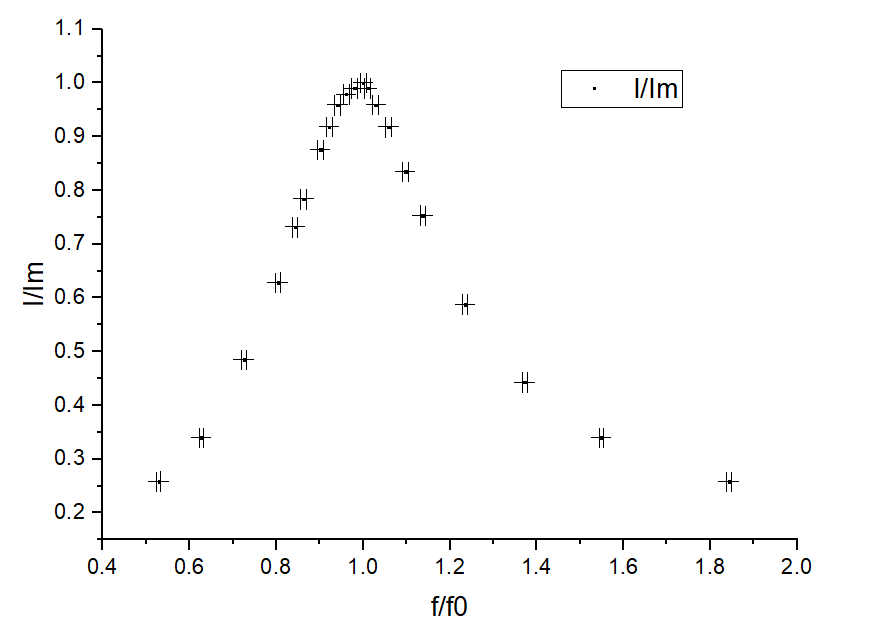
\includegraphics[width=0.7\textwidth]{o1} 
    \caption{Figure of $\frac{I}{I_{m}} \text { vs. } \frac{f}{f_{0}}$.} 
\end{figure}

\subsubsection{\textsc{phase-frequency characteristic (experimental)}}
The data and calculated values of amplitude-frequency characteristic are shown in Table 7, and the other uncertainties are shown in Table 5 above.

In Table 7, for sample calculation, we take $U_R = 1.00 [V_{pp}]$ with $U_m = 3.88 [V_{pp}]$. Then, we can calculate $\varphi_{\exp }$ as follows:

\begin{center}
$\varphi_{\exp }=\cos ^{-1}\left(\frac{U_{R}}{U_{m}}\right)=\cos ^{-1}(0.258)=1.310 \pm 0.006$
\end{center}

Then, we are able to use \textit{Origin} to plot the figure of $\displaystyle \varphi_{exp} \text { vs. } \frac{f}{f_{0}}$, which is shown in Fig.10.



\begin{table}[p]
\begin{center}
\begin{tabular}{|c|c|c|c|c|c|}
\hline
$U_R [V_{pp}] \pm 0.02 [V_{pp}] $ & f $[Hz] \pm 0.001[Hz]$ & $f/f_0$ & $u_{f/f_0}$ & $\varphi_{exp}$ & $u_{\varphi_{exp}}$ \\ \hline
1.00 & 2700.000 & 0.5294118 & 0.0000002 & 1.310 & 0.006 \\ \hline
1.32 & 3200.000 & 0.6274510 & 0.0000002 & 1.224 & 0.006 \\ \hline
1.88 & 3700.000 & 0.7254902 & 0.0000002 & 1.065 & 0.007 \\ \hline
2.44 & 4100.000 & 0.8039216 & 0.0000003 & 0.891 & 0.008 \\ \hline
2.84 & 4300.000 & 0.8431373 & 0.0000003 & 0.750 & 0.009 \\ \hline
3.04 & 4400.000 & 0.8627451 & 0.0000003 & 0.671 & 0.011 \\ \hline
3.40 & 4600.000 & 0.9019608 & 0.0000003 & 0.503 & 0.014 \\ \hline
3.56 & 4700.000 & 0.9215686 & 0.0000003 & 0.409 & 0.018 \\ \hline
3.72 & 4800.000 & 0.9411765 & 0.0000003 & 0.29 & 0.03 \\ \hline
3.80 & 4900.000 & 0.9607843 & 0.0000003 & 0.20 & 0.04 \\ \hline
3.84 & 5000.000 & 0.9803921 & 0.0000003 & 0.14 & 0.05 \\ \hline
3.88 & 5100.000 & 1.0000000 & 0.0000003 & 0 & / \\ \hline
3.84 & 5150.000 & 1.0098039 & 0.0000003 & 0.14 & 0.05 \\ \hline
3.72 & 5250.000 & 1.0294118 & 0.0000003 & 0.29 & 0.03 \\ \hline
3.56 & 5400.000 & 1.0588235 & 0.0000003 & 0.409 & 0.018 \\ \hline
3.24 & 5600.000 & 1.0980392 & 0.0000003 & 0.583 & 0.012 \\ \hline
2.92 & 5800.000 & 1.1372549 & 0.0000003 & 0.719 & 0.010 \\ \hline
2.28 & 6300.000 & 1.2352941 & 0.0000003 & 0.943 & 0.007 \\ \hline
1.72 & 7000.000 & 1.3725490 & 0.0000003 & 1.112 & 0.006 \\ \hline
1.32 & 7900.000 & 1.5490196 & 0.0000004 & 1.224 & 0.006 \\ \hline
1.00 & 9400.000 & 1.8431373 & 0.0000004 & 1.310 & 0.006 \\ \hline
\end{tabular}
\caption{Measurement Data for phase-frequency characteristic (experimental).}
\end{center}
\end{table}

\newpage
\begin{figure}[htb] 
    \centering
    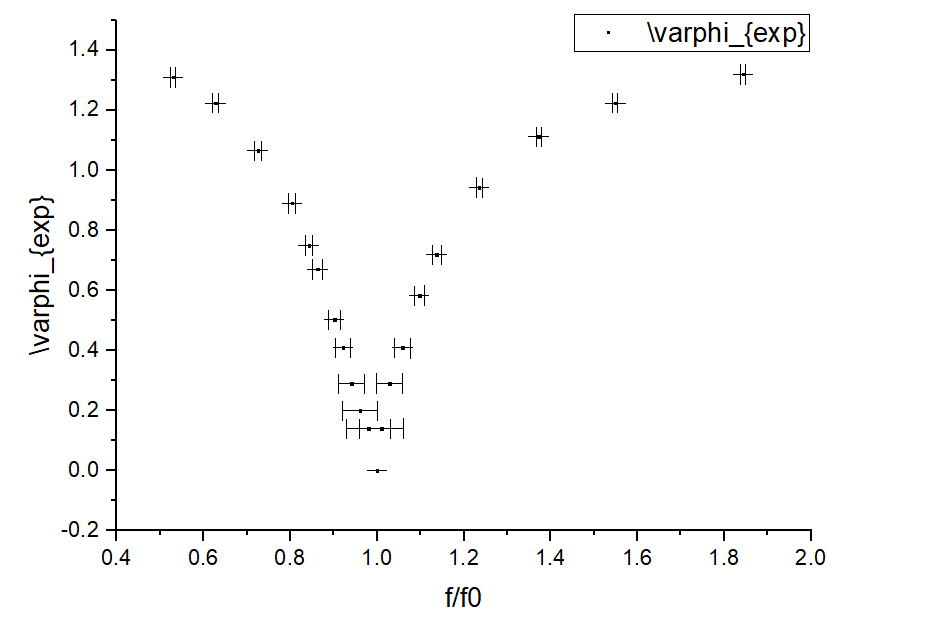
\includegraphics[width=0.7\textwidth]{o2} 
    \caption{Figure of $\varphi_{exp} \text { vs. } \frac{f}{f_{0}}$.} 
\end{figure}

\subsubsection{\textsc{phase-frequency characteristic (theoretical)}}
The data and calculated values of amplitude-frequency characteristic are shown in Table 8, and the other uncertainties are shown in Table 5 above.

In Table 8, for sample calculation, we take $f = 2700.000[Hz] $. Then, we can calculate $\varphi_{\exp }$ as follows:

\begin{center}
$\begin{aligned} \varphi_{\text {theo}} &=\tan ^{-1}\left(\frac{\omega L-\frac{1}{\omega C}}{R}\right)\\ 
&=\tan ^{-1}\left(\frac{2 \pi L f-\frac{1}{2 \pi C f}}{R}\right) \\ 
	&=\tan ^{-1}\left(\frac{\left.2 \pi \times 0.01 \times 2700.000-\frac{1}{2 \pi \times 2700 \times 101.85 \times 10^{-9}}\right)}{99.90}\right) \\ &=-1.33129452 \pm 1.6 \times 10^{-7} \end{aligned}$
\end{center}

Then, we are able to use \textit{Origin} to plot the figure of $\displaystyle \varphi_{theo} \text { vs. } \frac{f}{f_{0}}$, which is shown in Fig.11.

\begin{table}[p]
\begin{center}
\begin{tabular}{|c|c|c|c|c|c|}
\hline
$U_R [V_{pp}] \pm 0.02 [V_{pp}] $ & f $[Hz] \pm 0.001[Hz]$ & $f/f_0$ & $u_{f/f_0}$ & $\varphi_{theo}$ & $u_{\varphi_{theo}}$ \\ \hline
1.00 & 2700.000 & 0.5294118 & 0.0000002 & -1.33129452 & $1.6\times 10^{-7}$ \\ \hline
1.32 & 3200.000 & 0.6274510 & 0.0000002 & -1.2361143 & $2\times 10^{-7}$ \\ \hline
1.88 & 3700.000 & 0.7254902 & 0.0000002 & -1.0864214 & $4\times 10^{-7}$ \\ \hline
2.44 & 4100.000 & 0.8039216 & 0.0000003 & -0.8907320 & $6\times 10^{-7}$ \\ \hline
2.84 & 4300.000 & 0.8431373 & 0.0000003 & -0.7508639 & $6\times 10^{-7}$ \\ \hline
3.04 & 4400.000 & 0.8627451 & 0.0000003 & -0.6671600 & $7\times 10^{-7}$ \\ \hline
3.40 & 4600.000 & 0.9019608 & 0.0000003 & -0.4694600 & $8\times 10^{-7}$ \\ \hline
3.56 & 4700.000 & 0.9215686 & 0.0000003 & -0.3561749 & $9\times 10^{-7}$ \\ \hline
3.72 & 4800.000 & 0.9411765 & 0.0000003 & -0.2353672 & $1.0\times 10^{-6}$ \\ \hline
3.80 & 4900.000 & 0.9607843 & 0.0000003 & -0.1099666 & $1.2\times 10^{-6}$ \\ \hline
3.84 & 5000.000 & 0.9803921 & 0.0000003 & 0.0163264 & $1.3\times 10^{-6}$ \\ \hline
3.88 & 5100.000 & 1.0000000 & 0.0000003 & 0.1396490 & $1.4\times 10^{-6}$ \\ \hline
3.84 & 5150.000 & 1.0098039 & 0.0000003 & 0.1991148 & $1.3\times 10^{-6}$ \\ \hline
3.72 & 5250.000 & 1.0294118 & 0.0000003 & 0.3120022 & $1.1\times 10^{-6}$ \\ \hline
3.56 & 5400.000 & 1.0588235 & 0.0000003 & 0.4633602 & $8\times 10^{-7}$ \\ \hline
3.24 & 5600.000 & 1.0980392 & 0.0000003 & 0.6298487 & $6\times 10^{-7}$ \\ \hline
2.92 & 5800.000 & 1.1372549 & 0.0000003 & 0.7602832 & $5\times 10^{-7}$ \\ \hline
2.28 & 6300.000 & 1.2352941 & 0.0000003 & 0.9764272 & $3\times 10^{-7}$ \\ \hline
1.72 & 7000.000 & 1.3725490 & 0.0000003 & 1.1386321 & $2\times 10^{-7}$ \\ \hline
1.32 & 7900.000 & 1.5490196 & 0.0000004 & 1.24790982 & $8\times 10^{-8}$ \\ \hline
1.00 & 9400.000 & 1.8431373 & 0.0000004 & 1.33960377 & $4\times 10^{-8}$ \\ \hline
\end{tabular}
\caption{Measurement Data for phase-frequency characteristic (theoretical).}
\end{center}
\end{table}

\newpage
\begin{figure}[htb] 
    \centering
    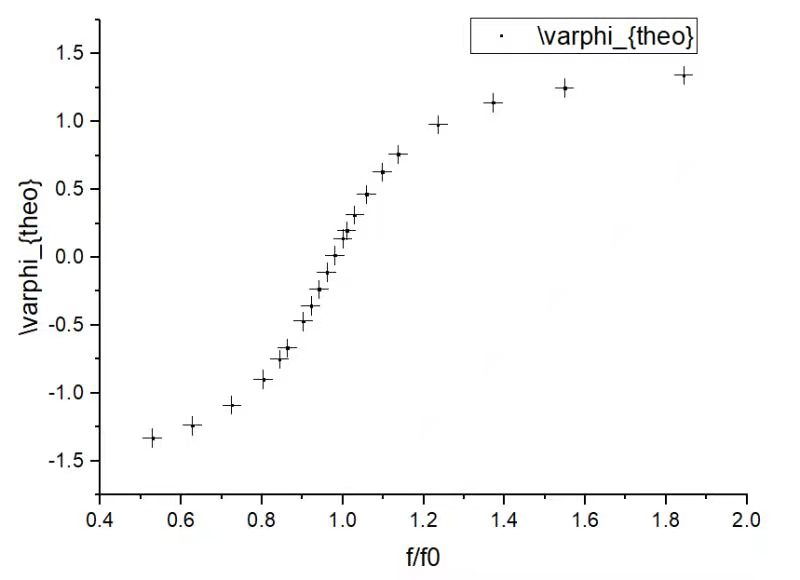
\includegraphics[width=0.7\textwidth]{o3} 
    \caption{Figure of $\varphi_{theo} \text { vs. } \frac{f}{f_{0}}$.} 
\end{figure}

\subsection{\textsc{Quality Factor}}
\subsubsection{\textsc{Experimental Quality Factor}}
To find out the experimental quality factor, we find the proper $f_1$ and$f_2$, such that $I(f_1) = I(f_2) = I_m/\sqrt{2}$. We can obtain the most suitable frequencies:
\begin{center}
$ f_1 = 4300.000 [Hz] $
\end{center}
and 
\begin{center}
$ f_1 = 5900.000 [Hz] $
\end{center}
Hence we obtain:
\begin{center}
$\displaystyle Q_{exp} = \frac{f_0}{f_2 - f_1} = \frac{5100.000}{5900.000 - 4300.000} = 3.187500 \pm 0.000003$
\end{center}
\subsubsection{\textsc{Theoretical Quality Factor}}
We obtain that:
\begin{center}
$\displaystyle Q_{theo} = \frac{\sqrt{LC}}{RC} = \frac{\sqrt{0.01 \times 101.85\times 10^{-9} }}{99.90 \times 101.85\times 10^{-9}} = 3.137 \pm 0.004$
\end{center}
\par The relative error between experimental and theoretical values can be calculated as:
\begin{center}
$\displaystyle u_Q =  \frac{3.187500 - 3.137}{3.137} = 1.6\% $
\end{center}
which is a satisfactory result.

%----------------------------------------------------------------------------------------
%	SECTION 6
%----------------------------------------------------------------------------------------
\newpage
\section{\textsc{Conclusion and Discussion}}
\subsection{\textsc{Discussion}}
In this lab, generally speaking, we do a great job and have some satisfactory results. We studied the properties of RC,LC,and RLC circuits. However, there still exists some errors. We will discussed them one by one.
\subsubsection{\textsc{Errors in RC SERIES CIRCUIT}}
In RC series circuit, our relative error reaches 13\%, which is too high. This may come from the misreading from me. In other words, I misread the $T_{1/2}$, which is actually $7.000[\mu s]$. This is because when I switch the knob, the value changes between $7.000[\mu s]$ and $8.000[\mu s]$, which makes me hard to decide which one I should choose to be my reading. 
\par Fortunately, the problem can be solved by changing the vertical scale of the waveform. As shown in Fig.12 (taken from VE215 Lab), the vertical scale is carefully changed so that the waveform becomes "larger" and more "friendly" for us to observe. In this case, it will be more likely for us to decide an accurate $T_{1/2}$ than the one in Fig.6.

\begin{figure}[htb] 
    \centering
    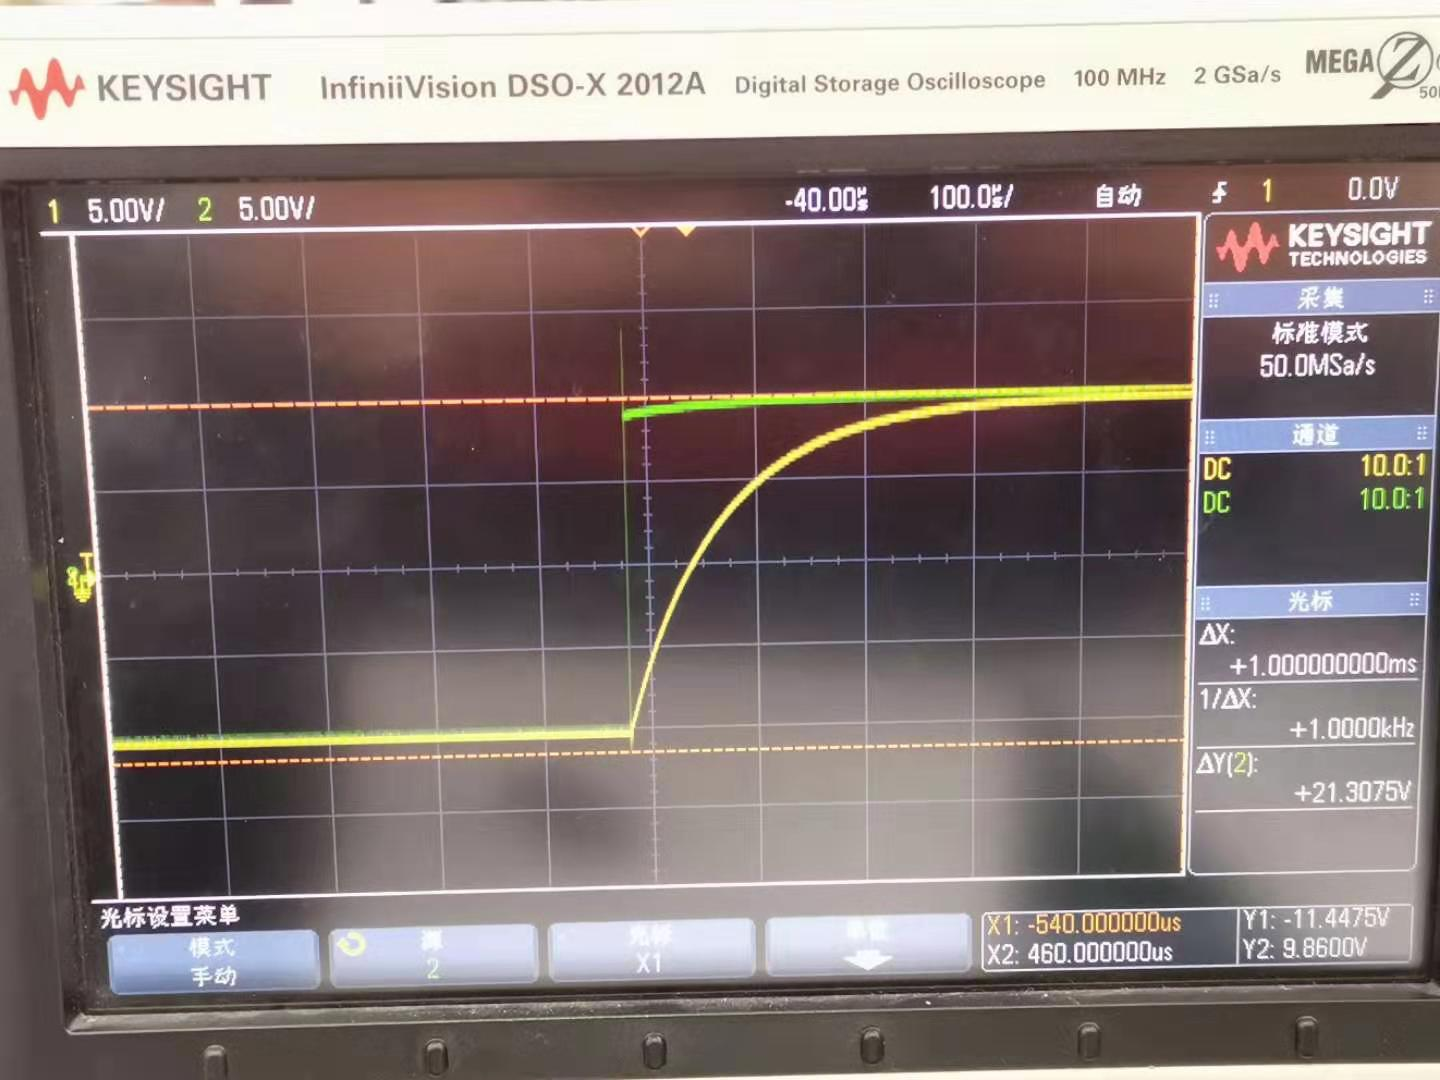
\includegraphics[width=0.5\textwidth]{d1} 
    \caption{Waveform with a different vertical scale.} 
\end{figure}

\subsubsection{\textsc{Errors in RL and RLC SERIES CIRCUIT}}
	In RLC circuit, our relative error is -7\%, which is large but acceptable. Some common errors may occurs, resulting in the error:
	\begin{itemize}
	\item[1.] The voltage in the oscilloscope is always oscillating and not stable.
	\item[2.] The protoboard and wires also have resistance, which we ignore in this lab.
	\item[3.] The resistance may change due to different temperature. Hence errors may occur.
	\item[4.] When discovering the critically damped case in RLC circuit, it's difficult for us to judge it by our eyes. Consequently, the result is not accurate.
	\end{itemize}

\subsubsection{\textsc{Errors in RLC Resonant Circuit, Quality Factor}}
	In this part, our results are overall satisfactory. Some minor sources of errors may be:
\begin{itemize}
	\item[1.] The voltage in the oscilloscope is always oscillating and not stable.
	\item[2.] The capacitor and inductor is not ideal.
	\item[3.] We assume that the uncertainty of the inductor is 0, which is not the case in real world.
	\end{itemize}
	
\subsubsection{\textsc{Suggestions}}
Hence, I put forward some suggestions, which may help the experiment be more successful:
\begin{itemize}
\item[1.] As we have discussed in 6.1.1, change the scale on the oscilloscope if necessary to have a more accurate reading.
\item[2.] Wait for several minutes so that the oscillation of the voltage across the oscilloscope becomes stable.
\item[3.] Take into consideration the uncertainty of the inductor, rather than simply taking it as "0".
\item[4.] Measure the resistance of the resistor exactly before or after the lab to avoid the influence of temperature.
\item[5.] Take into consideration the resistance of wires and inner structure of the protoboard.
\item[6.] In this lab, we may use higher voltage input. As a result, the oscillation may decrease, and the error decrease accordingly.
\item[7.] When calculating experimental quality factor, our $f_1$ and $f_2$ may have a large error. Hence, we may improve this by doing some calculations based on our result.
\item[8.] We may use computer to record the data to make the results more accurate.
\end{itemize}

\subsection{\textsc{Conclusion}}
In this lab, we really have learned a lot, we studied:
\begin{itemize}
\item[1.] The general idea of alternating-current circuits.
\item[2.] General RC, RL, and RLC circuit.
\item[3.] The concept of resonance circuit and quality factor.
\item[4.] How to measure the amplitude- frequency and the phase-frequency characteristics of circuits.
\item[5.] How to use oscilloscope.
\end{itemize}

%----------------------------------------------------------------------------------------
%	SECTION 7
%----------------------------------------------------------------------------------------

\begin{appendices} 
\section{\textsc{Measurement uncertainty analysis}} 
\subsection{\textsc{RC Series Circuit}}
Based on uncertainty propagation, the uncertainty for the experimental time constant $ \tau_{exp} $ can be found as:
\begin{center}
$ \displaystyle u_{\tau_{exp}} = \sqrt{(\frac{\partial \tau_{exp}}{\partial T_{1/2}})^2(u_{T_{1/2}})^2} = \frac{u_{T_{1/2}}}{\text{ln}2} = \frac{0.001\times 10^{-6}}{0.693} = 1.4 \times 10^{-9} [s] $
\end{center}
The uncertainty for the theoretical time constant $ \tau_{theo} $ can be found similarly:
\begin{center}
$ \displaystyle  
\begin{aligned} 
	u_{\tau_{theo}} &= \sqrt{(\frac{\partial \tau_{theo}}{\partial R})^2(u_R)^2 + (\frac{\partial \tau_{theo}}{\partial C})^2(u_C)^2} \\ 
		&= \sqrt{C^2~u_R^2 + R^2~u_C^2} \\ 
		&= \sqrt{(101.85 \times 10^{-9} \times 0.01)^2 + (99.90 \times 0.01 \times 10^{-9})^2} \\
		&= 1.4 \times 10^{-9} [s] 
\end{aligned}$
\end{center}

\subsection{\textsc{RL Series Circuit}}
Based on uncertainty propagation, the uncertainty for the experimental time constant $ \tau_{exp} $ can be found as:
\begin{center}
$ \displaystyle u_{\tau_{exp}} = \sqrt{(\frac{\partial \tau_{exp}}{\partial T_{1/2}})^2(u_{T_{1/2}})^2} = \frac{u_{T_{1/2}}}{\text{ln}2} = \frac{0.01\times 10^{-6}}{0.693} = 1.4 \times 10^{-8} [s] $
\end{center}
The uncertainty for the theoretical time constant $ \tau_{theo} $ can be found similarly:
\begin{center}
$ \displaystyle  
\begin{aligned} 
	u_{\tau_{theo}} &= \sqrt{(\frac{\partial \tau_{theo}}{\partial R})^2(u_R)^2 + (\frac{\partial \tau_{theo}}{\partial L})^2(u_L)^2} \\ 
		&= \frac{L}{R^2}~u_R \\ 
		&= \frac{0.01}{99.90^2}\times 0.01 \\
		&= 1.0 \times 10^{-8} [s] 
\end{aligned}$
\end{center}

\subsection{\textsc{RLC Series Circuit}}
Based on uncertainty propagation, the uncertainty for the experimental time constant $ \tau_{exp} $ can be found as:
\begin{center}
$ \displaystyle u_{\tau_{exp}} = \sqrt{(\frac{\partial \tau_{exp}}{\partial T_{1/2}})^2(u_{T_{1/2}})^2} = \frac{u_{T_{1/2}}}{\beta t} = \frac{0.01\times 10^{-6}}{1.68} = 6 \times 10^{-9} [s] $
\end{center}
The uncertainty for the theoretical time constant $ \tau_{theo} $ can be found similarly:
\begin{center}
$ \displaystyle  
\begin{aligned} 
	u_{\tau_{theo}} &= \sqrt{(\frac{\partial \tau_{theo}}{\partial C})^2(u_C)^2 + (\frac{\partial \tau_{theo}}{\partial L})^2(u_L)^2} \\ 
		&= \frac{\sqrt{L}}{2\sqrt{C}}~u_C \\ 
		&= \frac{\sqrt{0.01}}{2 \times \sqrt{101.85\times 10^{-9}}}\times 0.01 \times 10^{-9} \\
		&= 1.6 \times 10^{-9} [s] 
\end{aligned}$
\end{center}

\subsection{\textsc{RLC Resonant Circuit}}
\subsubsection{\textsc{Amplitude-frequency characteristic}}
Based on uncertainty propagation, since $I/I_m = U/U_m$, the uncertainty for $u_{I/I_m}$ can be found as:
\begin{center}
$ \displaystyle  
\begin{aligned} 
	u_{I/I_m} &= u_{U/U_m} = \sqrt{(\frac{\partial \frac{U}{U_m}}{\partial U})^2(u_U)^2 + (\frac{\partial \frac{U}{U_m}}{\partial U_m})^2(u_{U_m})^2} \\
		&= \sqrt{(\frac{u_U}{U_m})^2 + (\frac{U\times u_{U_m}}{U_m^2})^2} \\ 
\end{aligned}$
\end{center}
For sample calculations, we choose $U_R = 1.00 [V_{pp}]$ and $f = 2700.000[Hz]$, and we will have:
\begin{center}
$ \displaystyle  
\begin{aligned} 
	u_{I/I_m} &= \sqrt{(\frac{0.02}{3.88})^2 + (\frac{1.00 \times 0.02}{3.88^2})^2} = 0.005\\ 
\end{aligned}$
\end{center}

Based on uncertainty propagation, the uncertainty for $u_{f/f_0}$ can be found as:
\begin{center}
$ \displaystyle  
\begin{aligned} 
	u_{f/f_0} &= \sqrt{(\frac{\partial \frac{f}{f_0}}{\partial f})^2(u_f)^2 + (\frac{\partial \frac{f}{f_0}}{\partial f_0})^2(u_{f_0})^2} \\
		&= \sqrt{(\frac{u_f}{f_0})^2 + (\frac{f\times u_{f_0}}{f_0^2})^2} \\ 
\end{aligned}$
\end{center}
For sample calculations, we choose $f = 2700.000 [V]$ and $f_0 = 5100.000[Hz]$, and we will have:
\begin{center}
$ \displaystyle  
\begin{aligned} 
	u_{f/f_0} &= \sqrt{(\frac{0.001}{5100.000})^2 + (\frac{2700.000 \times 0.001}{5100.000^2})^2} = 2\times 10^{-7}\\ 
\end{aligned}$
\end{center}

\subsubsection{\textsc{phase-frequency characteristic (experimental)}}
In this section, what we need to calculate more is $\varphi_{exp}$. It can be calculated as follows (Take $U_R = 1.00[V_{pp}]$ and $U_m = 3.88[V_{pp}]$ as a sample calculation):
\begin{center}
$\begin{aligned}
u_{\varphi_{\exp }} &=\sqrt{\left(\frac{\partial \varphi_{\exp }}{\partial U_{R}}\right)^2 \left(u_{U_{R}}\right)^{2}+\left(\frac{\partial \varphi_{\exp }}{\partial U_{m}}\right)^2 \left( u_{U_{m}}\right)^{2}} \\ 
%		&=\sqrt{\left( \frac{u_{U_{R}}}{U_{m} \frac{U_{R}}{\sqrt{1-U_{m}}}}\right)^2 + \left(\frac{u_{U_{m}} 
%       U_{R}}{U_{m}^{2}\sqrt{\frac{U_{R}^{2}}{U_{m}^{2}-1}}}\right)^2} \\ 	
	&=\sqrt{\frac{u_{U_{R}}^{2}}{U_{m}^{2} \left(1- \frac{U_R^2}{U_m^2} \right)}+\frac{u_{U_{m}}^{2} U_{R}^{2}}{U_{m}^{4}\left( 1-\frac{U_R^2}{U_m^2} \right)}} \\ 
	&=0.006\text{\quad(Plugging in } U_R = 1.00[V_{pp}] \text{ and } U_m = 3.88[V_{pp}]\text{)} \end{aligned}$
\end{center}

\subsubsection{\textsc{phase-frequency characteristic (theoretical)}}
In this section, what we need to calculate more is $\varphi_{exp}$. It can be calculated as follows (Take $f = 2700[Hz]$ as a sample calculation):
\begin{center}
\begin{scriptsize}
$\begin{aligned}
u_{\varphi_{theo }} &=\sqrt{\left(\frac{\partial \varphi_{\text {theo}}}{\partial U_{f}} \times u_{U_{f}}\right)^{2}+\left(\frac{\partial \varphi_{\text {theo}}}{\partial L} \times u_{L}\right)^{2}+\left(\frac{\partial \varphi_{\text {theo}}}{\partial C} \times u_{C}\right)^{2}+\left(\frac{\partial \varphi_{\text {theo}}}{\partial R} \times u_{R}\right)^{2}} \\ 
	&=\sqrt{ \left(\frac{(2\pi L + \frac{1}{2\pi Cf^2})~u_f}{1 + \frac{(2\pi Lf-\frac{1}{2\pi fC})^2}{R^2}}\right)^2 + \left(  \frac{2\pi f u_L}{1+\frac{\left(  2\pi f L - \frac{1}{2\pi fC}  \right)^2}{R^2}}  \right)^2 + \left(  \frac{u_C}{2fC^2R \left(  1 + \frac{(2\pi Lf -\frac{1}{2\pi Cf})^2}{R^2}  \right)}  \right)^2  + \left(\frac{(2f\pi L - \frac{1}{2\pi fC})u_R}{1+\frac{\left(  2\pi f -\frac{1}{2\pi fC}  \right)^2}{R^2}}   \right)^2} \\ 
	&=1.6 \times 10^{-7} 
\end{aligned}$
\end{scriptsize}
\end{center}

\subsection{\textsc{Quality Factor}}
With the help of uncertainty propagation, we can find out $u_{Q_{e x p}} $:
\begin{center}
$\begin{aligned} u_{Q_{e x p}} 
	&=\sqrt{\left(\frac{\partial Q}{\partial f_{2}}  u_{f_{2}}\right)^{2}+\left(\frac{\partial Q}{\partial f_{1}}  u_{f_{1}}\right)^{2} + \left(\frac{\partial Q}{\partial f_{0}}  u_{f_{0}}\right)^{2}} \\ 
	&=\sqrt{\left(\frac{f_{0} \times u_{f_{2}}}{\left(f_{2}-f_{1}\right)^{2}}\right)^{2}+\left(\frac{f_{0} \times u_{f_{1}}}{\left(f_{2}-f_{1}\right)^{2}}\right)^{2} + \left(\frac{u_{f_{0}}}{f_{2}-f_{1}}\right)^{2}} \\ 
	&=3 \times 10^{-6} \end{aligned}$
\end{center}
\par Similarly, we are able to find out $u_{Q_{theo}}$ with the help of Mathematica:
\begin{center}
$u_{Q_{t h e o}}=\sqrt{\left(\frac{\partial Q}{\partial R} \times u_{R}\right)^{2}+\left(\frac{\partial Q}{\partial L} \times u_{L}\right)^{2}+\left(\frac{\partial Q}{\partial C} \times u_{C}\right)^{2}}=0.004$
\end{center}

\section{\textsc{Data sheet}} 
See the attached data sheet.
\end{appendices} 

%----------------------------------------------------------------------------------------
%	BIBLIOGRAPHY
%----------------------------------------------------------------------------------------

\begin{thebibliography}{9}
\bibitem{labmanual} Krzyzosiak, M. \& VP241 TA Groups.
\textit{Exercise 5 - lab manual [rev 4.3].pdf}. 
2019.
\end{thebibliography}


%----------------------------------------------------------------------------------------


\end{document}
